\begin{center}
    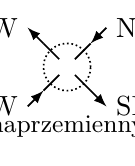
\begin{tikzpicture}[baseline=-0.65ex, scale=0.1]
    \useasboundingbox (-5, -9) rectangle (5, 5);
        \node [left] at (-5, -5) {SW};
        \draw[semithick,latex-] (-3, -3) to (-5,-5);
        \draw[semithick] (-3, -3) to (-1,-1);
        \node [right] at (5, 5) {NE};
        \draw[semithick,latex-] (3, 3) to (5,5);
        \draw[semithick] (3, 3) to (1,1);
        \node [right] at (5, -5) {SE};
        \draw[semithick,-latex] (3, -3) to (5,-5);
        \draw[semithick] (3, -3) to (1,-1);
        \node [left] at (-5, 5) {NW};
        \draw[semithick,-latex] (-3, 3) to (-5,5);
        \draw[semithick] (-3, 3) to (-1,1);
        \draw[semithick, densely dotted] (-0, 0) circle (3);
        \node at (0, -5) [below] {\small naprzemienny};
    \end{tikzpicture}
    \quad\quad\quad\quad\quad\quad
    \begin{tikzpicture}[baseline=-0.65ex, scale=0.1]
    \useasboundingbox (-5, -9) rectangle (5, 5);
        \node [left] at (-5, -5) {SW};
        \draw[semithick,latex-] (-3, -3) to (-5,-5);
        \draw[semithick] (-3, -3) to (-1,-1);
        \node [right] at (5, 5) {NE};
        \draw[semithick,-latex] (3, 3) to (5,5);
        \draw[semithick] (3, 3) to (1,1);
        \node [right] at (5, -5) {SE};
        \draw[semithick,latex-] (3, -3) to (5,-5);
        \draw[semithick] (3, -3) to (1,-1);
        \node [left] at (-5, 5) {NW};
        \draw[semithick,-latex] (-3, 3) to (-5,5);
        \draw[semithick] (-3, 3) to (-1,1);
        \draw[semithick, densely dotted] (-0, 0) circle (3);
        \node at (0, -5) [below] {\small sąsiadujący};
    \end{tikzpicture}
\end{center}